%% ==============
\chapter{Plannung der User Studie}
\label{ch:UserStudie}
%% ==============

Die Erkundungsphase, in der ein �berblick �ber das System und dessen
Komponenten gegeben wird, kann mit Hilfe eine Online-Konfigurators
ersetzt werden. Dem Benutzer wird das System im ganzen Pr�sentiert und
er hat die M�glichkeit die Komponenten auszuw�hlen die ihn
interessieren. Wird der Konfigurator benutzt kann automatisch f�r
jeden Kunden eine Feature-Liste erstellt werden. Aus dieser
Feature-Liste entsteht eine Variante des Produktes aus der das
Handbuch generiert werden soll.

%% ==============
\section{User Stories}
\label{ch:UserStudie}
%% ==============
User buys some of the gizmos we offer
In the background the configuration has to check the constraints
User gets the package and a QR code to read in with the app(offline for mounting when data connection available)



%===========PPT
Wizard of Oz
Standard Handbuch vs. individuell zugeschneidertes

Szenario
Konfigurationsportal zum Ausw�hlen der gew�nschten Komponenten
Nach der Auswahl werden individuelle Handb�cher erstellt
Die Gruppen unterscheiden sich nur in dem Handbuch
Vielleicht in einem 2. Experiment auch durch das Portal

Aufbau
Limitierung des Budgets um eine variierte Konfiguration zu erhalten
An einem Ort, wie z.B. Living Labs oder bei dem Nutzer zu Hause wird die Installation durchgef�hrt

Gruppen festlegen
2 Gruppen mit der selben Aufgabe aber verschiedene Handb�cher
Selektion der Teilnehmer
Ist Alter ein wichtiger Faktor
Technologie sollte m�glichst allen Gruppen einen Nutzen bringen
Laut Nielsen sind 5 Teilnehmer in der Anfangsphase ausreichend
Sample Size festlegen
Sind hier online Berechnungsysteme gut?
http://www.surveysystem.com/
Referenzimplementierung der Handb�cher muss gemacht werden.
Ein Handbuch, das mit einem solchen System kommt erhalten und bei einer Gruppe einsetzen

Ziel
Erfahren ob Nutzer ein Custom Handbook interessieren w�rde
Personenbefragungen 
Das Einsatzszenario einer Intelligente Heimautomatisierung erkl�ren mit einer Individuell zugeschneiderten Bedienungsanleitung
Die emotionale Reaktion k�nnte signifikant sein
Bewertung des Interesses an einer solchen Technologie

\begin{figure}[htp]
\begin{center}
  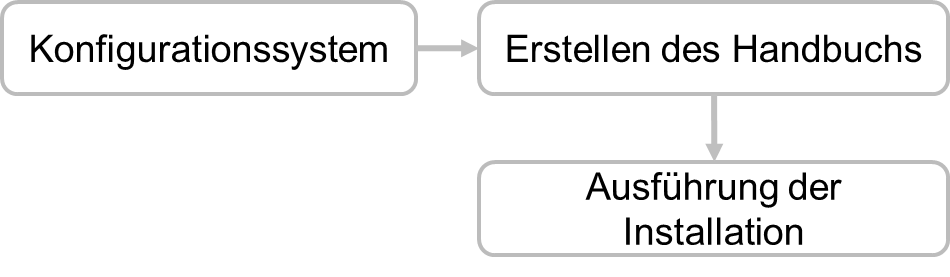
\includegraphics[width=1\textwidth]{img/studie-flowchart.png}
  \caption[labelInTOC]{figureCaption}
  \label{figureLabel}
\end{center}
\end{figure}

%============Wizard of Oz
Um eine Wizard of Oz Studie durchzuf�hren wird 
Es werden die Kommunikationsprotok
Keine Bus Technologien und alles was man in einer wiz of oz nicht sieht bzw.
nicht braucht. Keine Protokolle werden betrachtet.
We assume that the SW ist somehow deployed on the W.

Nutzer geht auf eine Webseite und w�hlt die Komponenten aus die er
ben�tigt. Dies ist der Konfigurationsschritt den der Nutzer
durchf�hrt. Mit den Konfigurationsdaten wird eine Instanz des
Modells angepasst. Diese Instanz soll dann mit Hilfe einer
Modelltransformation in Beschreibungsmodell transformiert werden.
Daraus soll zum Schluss eine nat�rlichsprachliche Benutzeranleitung
generiert werden.

 
%============Aufbau des Handbuches
Handbuch Metamodell?
Priorit�ten
Header/Footer
Struktur
IBM Decision Tree
I/O Felder
Hyperlinking
Welche Struktur sollte ein Handbuch haben
IBM Manual decision tree structure
How should the user be guided?
Hyperlinking?

%==============Aufbau Metamodell
There are two major types of control devices: devices that are produced to be 
flexibly adaptable to a wide range of tasks, and devices that are dedicated to 
a special purpose.

Es kann passieren, dass Nutzer wichtige Anweisungen �bersehen oder
nicht befolgen, daher w�re es n�tzlich diese hervorzuheben.

Metamodell sollte Assoziation und direktionalit�t in betracht nehmen
um erstens detailiertere Angaben �ber die Insallation zu geben wenn
ein Sensor kompliziert zu installieren ist oder viele Faktoren dort
einfliessen. Aber auch um die n�tigen Infomrationen zu enthalten um
die Fehlerfindung und bewertung der Insallation durchf�hren zu k�nnen.
Mass f�r komplexit�t:
direktionalit�t.


%============Durchzuf�hrende Aufgaben
 Die Aufgaben die bei der Installation durchzuf�hren sind:
 Home-Server platzieren,
 einschalten, Sensoren platzieren, assoziieren
 
 
 [Abh�ngigkeitsmatrix/Zusammenspiel aufzeigen? Ist ja das Wichtigste]
 
\begin{table}
  \caption{Elemente der Smart-Home Anwendung }
  \centering
  \begin{tabular}{l c c c c c}
    %heading
    \hline\hline
    
    Objekte & Aktuatoren & Sensoren  & Direktional & Proximit�t  \\   
    [1ex]

    \hline
    %heading end
    
	Fenster &  $\times$ & \checkmark \\ [1ex]
    
    Temperaturregler
    
    Anwendungsszenarien & & physiche Umgebung\\ [1ex]
    \hline
  \end{tabular}
  \label{table:smart-home-components}
\end{table}
 
  
%============Bewertung der Installation

Um die Installation bewerten zu k�nnen muss eine korrekte Definition
der Installation gegeben werden. Um die Bewertung durchzuf�hren werden
die Assozierung, Positionierung, Konfigurierung und weiter Aspekte in
betracht gezogen.
Folgende Tabelle zeigt es ausf�hrlich 
